%%%%%%%%%%%%%%%%%%%%%%%%%%%%%%%%%%%%%%%%%
% Beamer Presentation
% LaTeX Template
% Version 1.0 (10/11/12)
%
% This template has been downloaded from:
% http://www.LaTeXTemplates.com
%
% License:
% CC BY-NC-SA 3.0 (http://creativecommons.org/licenses/by-nc-sa/3.0/)
%
%%%%%%%%%%%%%%%%%%%%%%%%%%%%%%%%%%%%%%%%%

%----------------------------------------------------------------------------------------
%	PACKAGES AND THEMES
%----------------------------------------------------------------------------------------

\documentclass{beamer}
\usepackage[latin1]{inputenc}
\usepackage{multirow}
\usepackage{amsmath}

\mode<presentation> {

% The Beamer class comes with a number of default slide themes
% which change the colors and layouts of slides. Below this is a list
% of all the themes, uncomment each in turn to see what they look like.

%\usetheme{default}
%\usetheme{AnnArbor}
%\usetheme{Antibes}
%\usetheme{Bergen}
%\usetheme{Berkeley}
%\usetheme{Berlin}
%\usetheme{Boadilla}
%\usetheme{CambridgeUS}
%\usetheme{Copenhagen}
%\usetheme{Darmstadt}
%\usetheme{Dresden}
%\usetheme{Frankfurt}
%\usetheme{Goettingen}
%\usetheme{Hannover}
%\usetheme{Ilmenau}
%\usetheme{JuanLesPins}
%\usetheme{Luebeck}
\usetheme{Madrid}
%\usetheme{Malmoe}
%\usetheme{Marburg}
%\usetheme{Montpellier}
%\usetheme{PaloAlto}
%\usetheme{Pittsburgh}
%\usetheme{Rochester}
%\usetheme{Singapore}
%\usetheme{Szeged}
%\usetheme{Warsaw}

% As well as themes, the Beamer class has a number of color themes
% for any slide theme. Uncomment each of these in turn to see how it
% changes the colors of your current slide theme.

%\usecolortheme{albatross}
%\usecolortheme{beaver}
%\usecolortheme{beetle}
%\usecolortheme{crane}
%\usecolortheme{dolphin}
%\usecolortheme{dove}
%\usecolortheme{fly}
%\usecolortheme{lily}
%\usecolortheme{orchid}
%\usecolortheme{rose}
%\usecolortheme{seagull}
%\usecolortheme{seahorse}
%\usecolortheme{whale}
%\usecolortheme{wolverine}

%\setbeamertemplate{footline} % To remove the footer line in all slides uncomment this line
%\setbeamertemplate{footline}[page number] % To replace the footer line in all slides with a simple slide count uncomment this line

%\setbeamertemplate{navigation symbols}{} % To remove the navigation symbols from the bottom of all slides uncomment this line
}

\usepackage{graphicx} % Allows including images
\usepackage{booktabs} % Allows the use of \toprule, \midrule and \bottomrule in tables

%----------------------------------------------------------------------------------------
%	TITLE PAGE
%----------------------------------------------------------------------------------------

\title[JCHARMING]{A Bug Reproduction Approach Based on Directed Model Checking and Crash Traces} % The short title appears at the bottom of every slide, the full title is only on the title page

\author[Mathieu Nayrolles]{\underline{Mathieu Nayrolles$^1$}, Wahab Hamou-Lhadj$^1$, Sofi\`ene Tahar$^2$ and Alf Larsson$^3$} % Your name
\institute[Concordia] % Your institution as it will appear on the bottom of every slide, may be shorthand to save space
{
$^1$Software Behaviour Analysis (SBA) Research Lab, ECE,  Concordia, Montr\'eal, Canada\\
$^2$Hardware Verification Group (HVG) Research Lab, ECE, Concordia, Montr\'eal, Canada \\
$^3$PLF System Management, R\&D Ericsson, Stockholm, Sweden \\
\medskip
\textit{mathieu.nayrolles@gmail.com, wahab.hamou-lhadj@concordia.ca, tahar@ece.concordia.ca, alf.larsson@ericsson.com} % Your email address
}
\date{May 2nd, 2016} % Date, can be changed to a custom date

\begin{document}

\begin{frame}
\titlepage % Print the title page as the first slide
\end{frame}


\begin{frame}
\frametitle{Context: Software are released with bugs.}

\begin{itemize}
\item Despite testing and verification, softwares are pledged to be released with latent bugs.
\vspace{0.3cm}
\item Latent bugs will cause field crashes / faillures.
\vspace{0.3cm}
\item Patching field faillures is challenging:
\begin{itemize}
\vspace{0.3cm}
\item We have to know about them.
\vspace{0.3cm}
\item Information is scarce and inconsistent
\vspace{0.3cm}
\item Most valuable information are the one that help to reproduce a bug [Bettenburg, 2008].
\end{itemize}
\end{itemize}
\end{frame}

\begin{frame}
\frametitle{Related Works: Current ways to reproduce a crash.}
\begin{columns}[c] % The "c" option specifies centered vertical alignment while the "t" option is used for top vertical alignment

\column{.45\textwidth} % Left column and width
\textbf{Record and replay}
\begin{itemize}
\item Instrumentation of source code
\item Record on-field execution
\item Replay in-house
\vspace{0.3cm}
\item Cheap \& easy to implement
\item Yield good results
\item Overhead (1\% to 1066\%) and privacy concerns
\vspace{0.3cm}
\item JRapture'00, BugNet'05, ReCrash'08
\end{itemize}


\column{.5\textwidth} % Left column and width

\textbf{In house crash reproduction}
\begin{itemize}
\item Core dump.
\item Forward Symbolic Execution.
\item Backward Symbolic Execution.
\vspace{0.3cm}
\item Yield average results.
\item NP-Compex Problem
\item Exponential learning curve.
\item Privacy concerns.
\vspace{0.3cm}
\item BugRedux'12, RECORE'13, STAR'13
\end{itemize}

\end{columns}
\end{frame}


%------------------------------------------------


\begin{frame}
\frametitle{JCHARMING: A different direction}
\begin{itemize}

\item Avoid code instrumentation
\begin{itemize}
\vspace{0.3cm}
\item 0\% overhead
\end{itemize}
\vspace{0.3cm}
\item Do no yield privacy concerns
\begin{itemize}
\vspace{0.3cm}
\item Scalable to real-world and industrial/proprietary software systems
\end{itemize}
\vspace{0.3cm}
\item Leverage the stack traces resulting from a crash
\begin{itemize}
\vspace{0.3cm}
\item More and more often present in bug reports
\end{itemize}
\vspace{0.3cm}
\item JCHARMING uses directed model checking and backward slicing.
\end{itemize}
\end{frame}

\begin{frame}
\frametitle{Prelimenaries: \textbf{Testing}, Model Checking and Directed Model Checking}

\begin{figure}
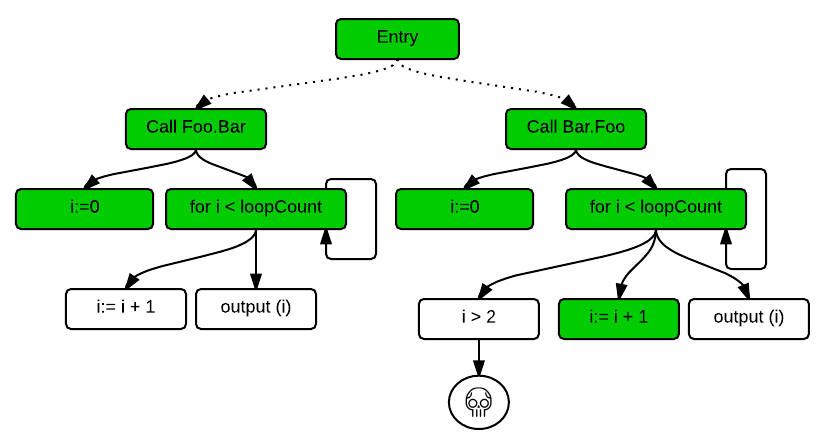
\includegraphics[width=0.75\linewidth]{media/test.png}
\end{figure}
\begin{itemize}
\item Depends on the tester understanding of the SUT.
\item Ineficient because it is not exhaustive.
\end{itemize}

\end{frame}

%------------------------------------------------

\begin{frame}
\frametitle{Prelimenaries: Model Checking}

\begin{itemize}

\item Checks if a given system under test (SUT) meets a specification $p$ by exhaustively testing every states. [Visser, 2003], [Kropf, 1999]
\end{itemize}
\begin{figure}
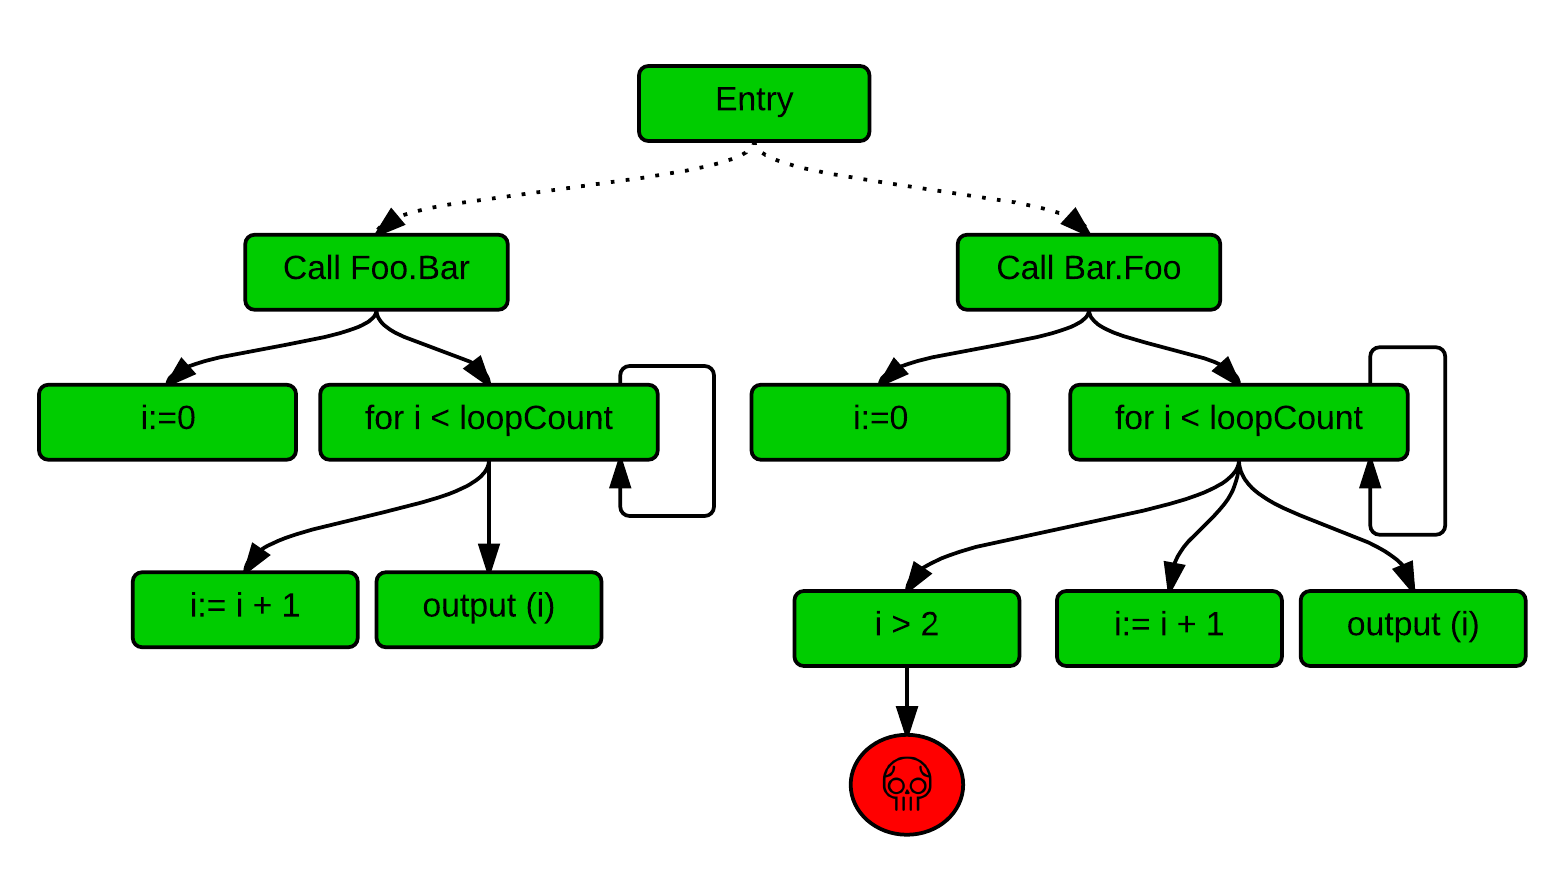
\includegraphics[width=0.4\linewidth]{media/mc.png}
\end{figure}

\begin{itemize}
\item Ensures that $p$ is reached at some point and not that $p$ holds nor $\forall x, p$ is satisfiable.
\item We aim to verify that $\forall$ states the program does not crash:

\end{itemize}

\begin{center}
$\forall x.(SUT, x) \models \neg c$
\end{center}

\begin{itemize}
\item Explores each and every state of the program, hence it is complete.
\item Impractical for real-world and large systems
\end{itemize}

\end{frame}

%------------------------------------------------



\begin{frame}
\frametitle{Prelimenaries: Testing, Model Checking and \textbf{Directed Model Checking}}

\begin{figure}
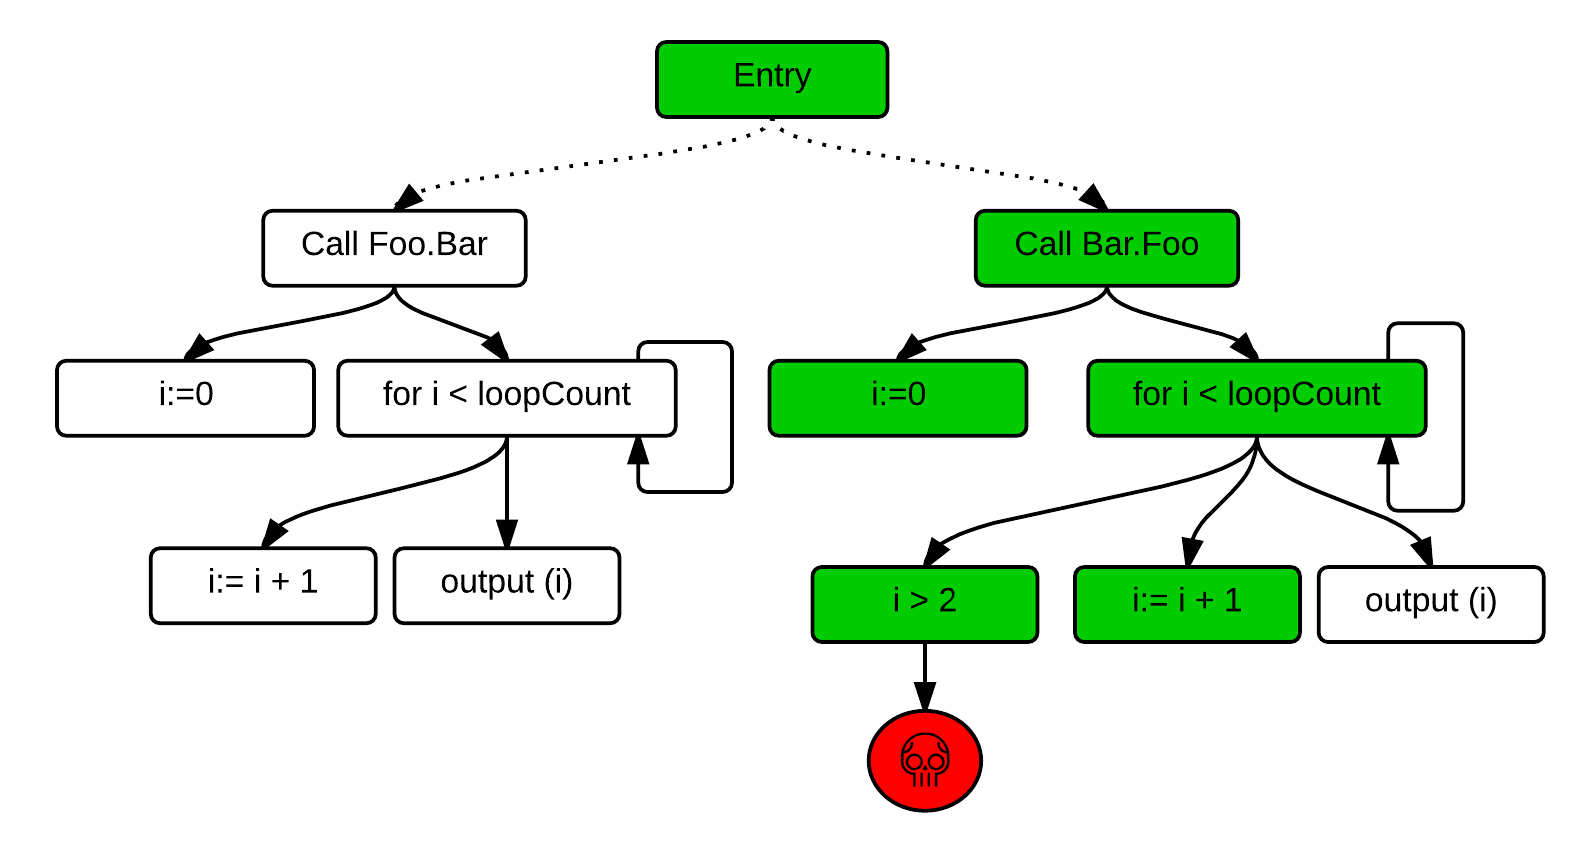
\includegraphics[width=0.75\linewidth]{media/dmc.png}
\end{figure}

\begin{itemize}
\item Explores only the states that may lead to a
specific location. [Rungta, 2009]
\item Use insights --- generally heuristics --- about the SUT to prune states.
\end{itemize}

\end{frame}

\begin{frame}
\frametitle{The JCHARMING approach}

\begin{figure}
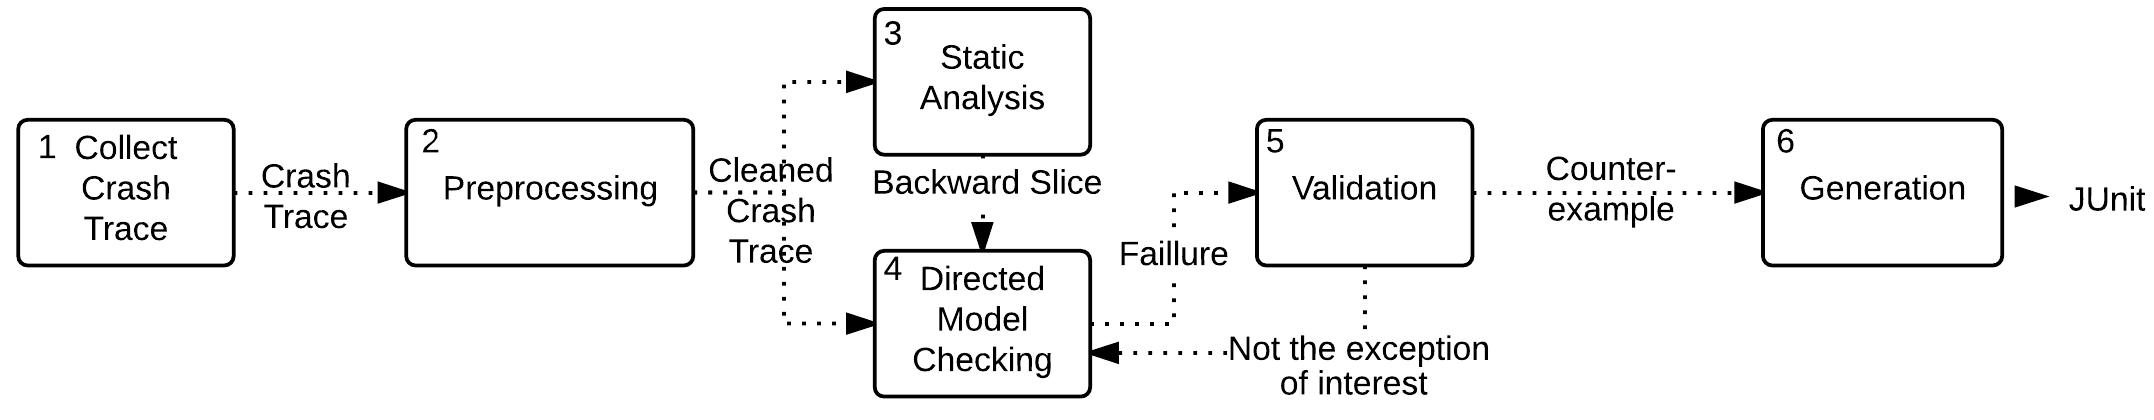
\includegraphics[width=0.97\linewidth]{media/approach.png}
\end{figure}

\begin{itemize}
\item \textbf{Step 1: Collect the crash trace}

\begin{small}
\texttt{1.javax.activity.IAE:loopTimes
should be < 3\\
2. at Foo.bar(Foo.java:10)\\
3. at GUI.buttonActionPerformed(GUI.java:88)\\
4. at GUI.access\$0(GUI.java:85)\\
5. at GUI\$1.actionPerformed(GUI.java:57)\\
6. caused by java.lang.IndexOutOfBoundsException : 3\\
7. at saner.Foo.buggy(Foo.java:17)\\
8. and 4 more ...\\}
\end{small}

\item \textbf{Step 2: Preprocessing}

\end{itemize}

\end{frame}

\begin{frame}

  \frametitle{Step 3: Building the Backward Static Slice (Cont'd)}

\begin{itemize}
  \item A backward slice contains all possible branches that may lead to a point $n$ from a point $m$ as well as the definition of the variables that control these branches
  \item Let's assume we have $T = \{k, i, f, d, b, c\}$
  \item Without using $T$ the backward slice is $\{a, b, d, e, h, u, j, k\}$.
  \item With $T$, and frame by frame it is $\{a, b, d, h, i, j, k\}$.
\end{itemize}

  \begin{figure}
  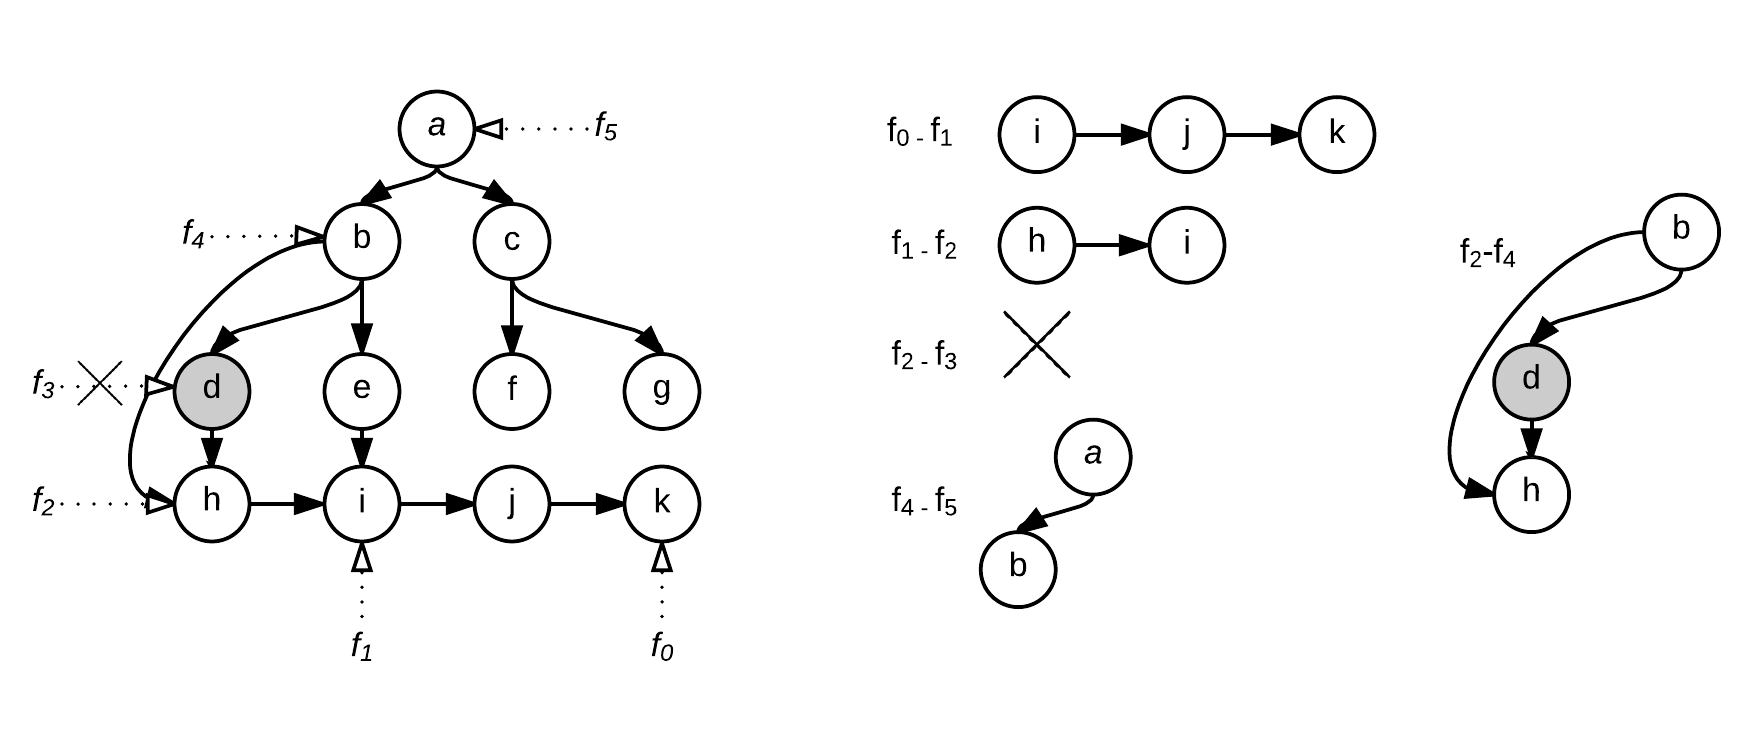
\includegraphics[width=\linewidth]{media/jcharming-slicing.png}
  \end{figure}

\end{frame}


\begin{frame}
\frametitle{Step 4: Directed Model Checking}

\begin{itemize}

\item We use Java PathFinder (JPF)
\begin{itemize}
\item JVM for Java bytecode verification.
\item Front-end for the SPIN model checker.
\item Developped and maintained by NASA.
\end{itemize}



\item Generate states
\item Forward

\begin{itemize}
\item Generates the next state $S_{t+1}$ and add it to the backtrack table
\end{itemize}

\item Backward

\item Backtrack
\begin{itemize}
\item Restore the last state of the backtrack table.
\end{itemize}

\item Restore state

\item Check properties

\begin{itemize}
\item Is triggered after each forward, backward and restore operations.
\end{itemize}


\end{itemize}

\end{frame}

\begin{frame}
\frametitle{Step 4: Directed Model Checking (Cont'd)}

\begin{itemize}


\item We modified the \textit{generate states} and the \textit{forward steps}.
\item The \textit{generate states} is populated with: $\bigcup_{i=0}^{entry} bslice_{[f_{i+1} \leftarrow f_i]} \, \subset \, SUT$
\item The \textit{foward step} can explore a state if $s_{i+1}$ and the transition $x$ from $s_i$ to $s_{i+1}$ are in $\bigcup_{i=0}^{entry} bslice_{[f_{i+1} \leftarrow f_i]} \, \subset \, SUT$

\item The \textit{check properties} step of JPF:

\begin{itemize}
\item If the current states transitions $x$ yield an exception
\item We execute $x$ and compare the stack trace to the original
\item If the two exceptions match, the bug is \textit{reproduced}.
\end{itemize}
\vspace{0.3cm}
\item JPF is now directed and explores only a sub-system of the SUT.
\end{itemize}

\end{frame}


\begin{frame}
\frametitle{Step 6: Generating Test Cases for Bug Reproduction}


  \begin{figure}
  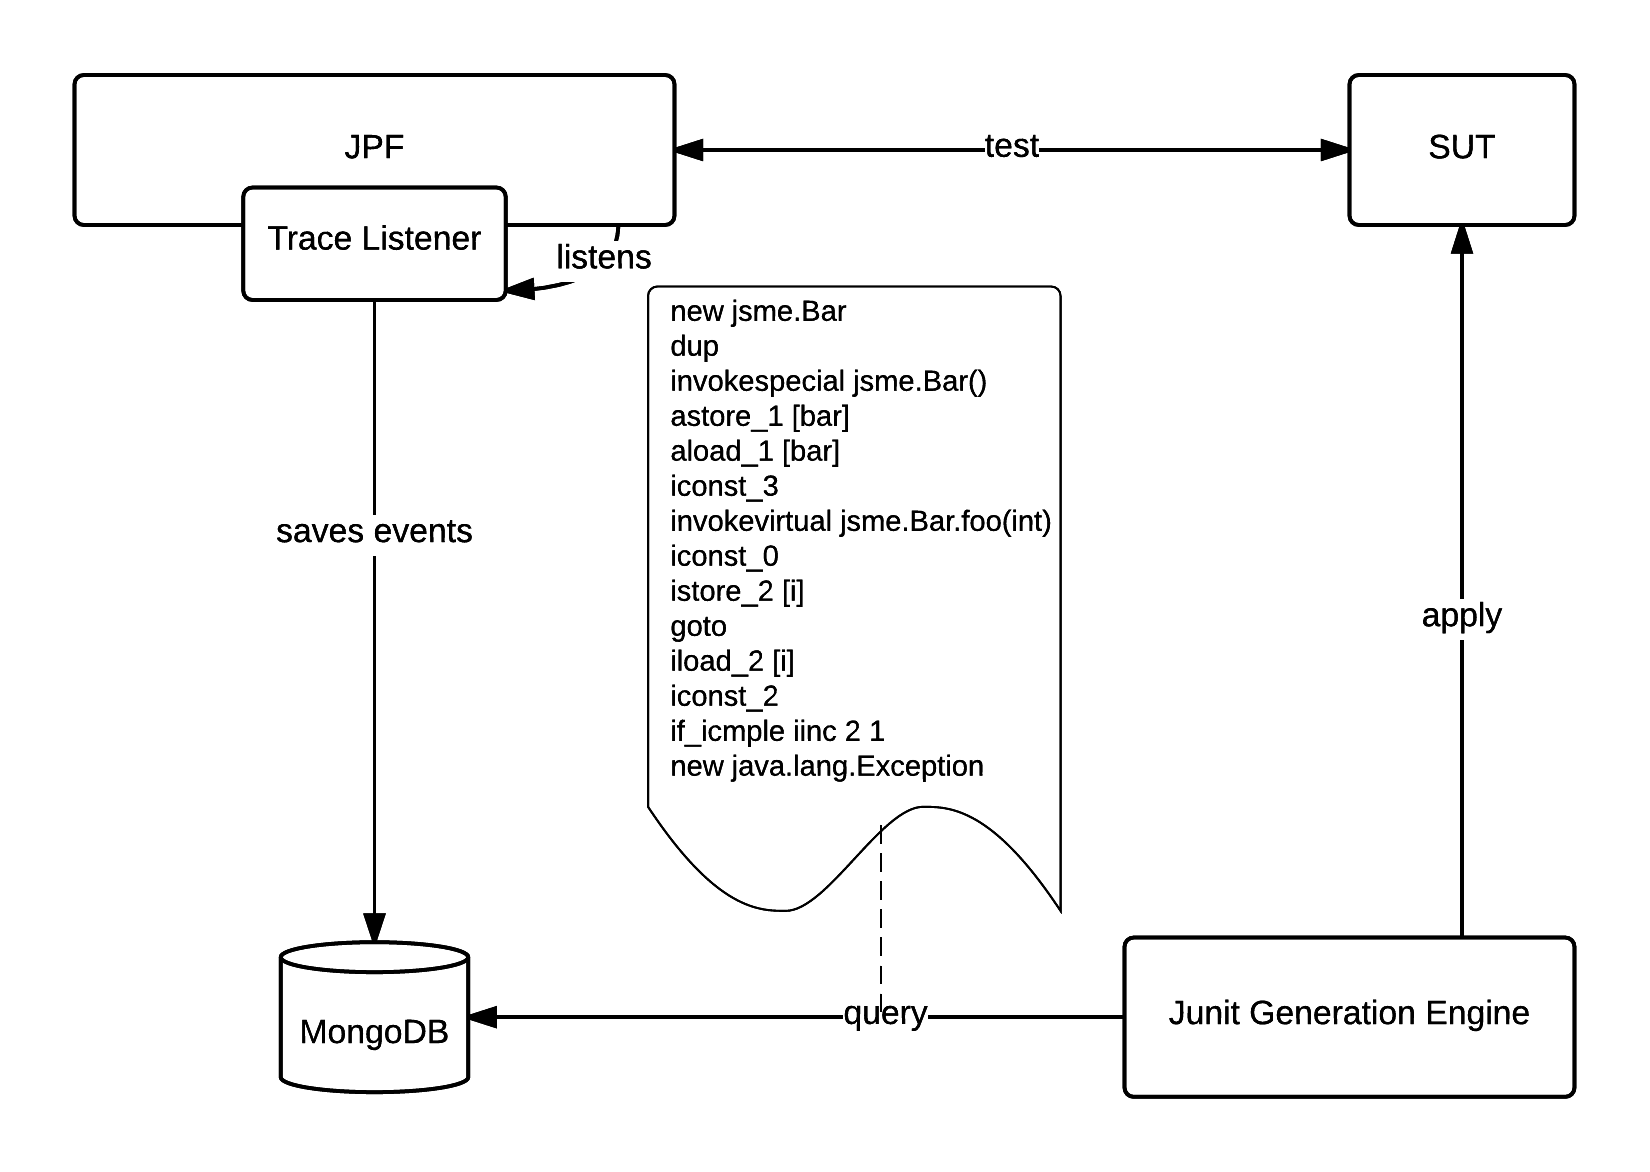
\includegraphics[width=0.95\linewidth]{media/unittest.png}
  \end{figure}


\end{frame}

\begin{frame}
\frametitle{Experiments And Conclusion}

\begin{itemize}
  \item 30 bugs belonging to 10 open sources systems (Ant, ArgoUML, DnsJava, jFreeChart, Log4j, MCT, PDFBox, Mahout, Hadoop, ActiveMQ).
  \item 80\% success ratio (24/30).
  \item Average success time is 19 minutes.
  \item Average fail time is 11 minutes.
  \item Average JUNIT length is 5 java statements.

  \vspace{0.5cm}
  \item Stress JCHARMING with more bugs
  \item Test the performances of JCHARMING with multi-threading related bugs
\end{itemize}

\end{frame}

%------------------------------------------------

\begin{frame}
\Huge{\centerline{QUESTIONS?}}
\end{frame}

%----------------------------------------------------------------------------------------

\end{document}
